\documentclass[xetex,mathserif,serif]{beamer}
\usepackage{polyglossia}
\setdefaultlanguage[babelshorthands=true]{russian}
\usepackage{minted}
\usepackage{tabu}
\usepackage[11pt]{moresize}

\useoutertheme{infolines}

\usepackage{fontspec}
\setmainfont{FreeSans}
\newfontfamily{\russianfonttt}{FreeSans}

\usepackage{textpos}
\setlength{\TPHorizModule}{1cm}
\setlength{\TPVertModule}{1cm}

\definecolor{links}{HTML}{2A1B81}
\hypersetup{colorlinks,linkcolor=,urlcolor=links}

\tabulinesep=0.7mm

\newcommand{\attribution}[1] {
    \vspace{-5mm}\begin{flushright}\begin{scriptsize}\textcolor{gray}{\textcopyright\, #1}\end{scriptsize}\end{flushright}
}

\title{Практика 14: REST-сервис}
\author[Юрий Литвинов]{Юрий Литвинов \newline \textcolor{gray}{\small\texttt{yurii.litvinov@gmail.com}}}

\date{25.04.2022}

\begin{document}

    \frame{\titlepage}

    \section{Краткий ликбез по веб-сервисам}

    \begin{frame}
        \frametitle{Как всё устроено}
        \begin{center}
            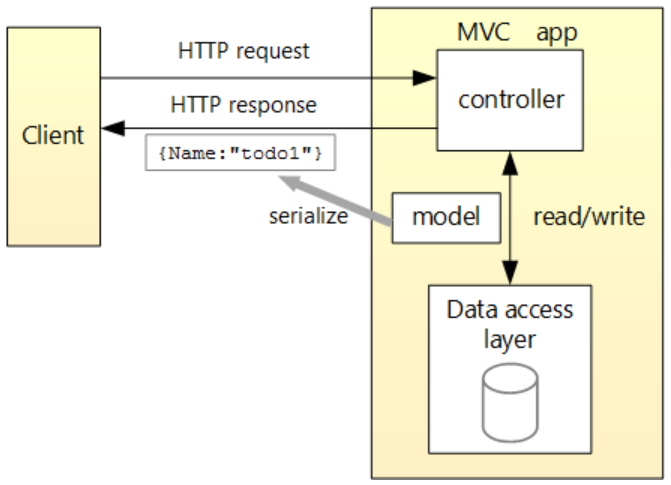
\includegraphics[width=0.4\textwidth]{webApiServiceDesign.png}
            \attribution{https://docs.microsoft.com/en-us/aspnet/core/tutorials/first-web-api}
        \end{center}
    \end{frame}

    \begin{frame}
        \frametitle{Как это делать в Visual Studio}
        \begin{itemize}
            \item Проект по шаблону ``ASP.NET Core Web API''
            \begin{itemize}
                \item Это тот же ASP.NET, но без View
            \end{itemize}
            \item Настройки по умолчанию
            \begin{itemize}
                \item Обратите внимание на поддержку OpenAPI
            \end{itemize}
            \item В папке Controllers собственно контроллеры
            \item Модели и бизнес-логика --- где угодно, но лучше сгруппировать
            \begin{itemize}
                \item Models для моделей
            \end{itemize}
        \end{itemize}
    \end{frame}

    \section{Задача}

    \begin{frame}
        \frametitle{Задача на пару}
        В командах по два человека спроектировать и реализовать REST-сервис, позволяющий интегрироваться с MyHwProj внешним системам.
        \begin{itemize}
            \item Потенциальные случаи использования:
            \begin{itemize}
                \item Реализация внешнего клиента для студента или преподавателя
                \item Сервис, выполняющий агрегацию и анализ статистики по курсу
            \end{itemize}
            \item Авторизация не нужна, считаем, что вся информация открыта
            \begin{itemize}
                \item Как в исходном задании, можно считать, что API преподавателя и студента доступны по разным URL
            \end{itemize}
            \item Используйте захардкоженные данные, реализация бизнес-логики не нужна
            \item Используйте Swagger или SoapUI для тестирования
            \begin{itemize}
                \item И попробуйте выполнить какой-нибудь GET-метод из браузера
            \end{itemize}
            \item Может помочь \url{https://docs.microsoft.com/en-us/aspnet/core/tutorials/first-web-api}
        \end{itemize}
    \end{frame}

\end{document}